\chapter{Running PyLith}
\label{cha:running}

\section{Organization of Simulation Components}

The components in a PyLith simulation generally fall into four main
categories:
\begin{description}
\item[Topology] Components associated with the spatial discretization
  of the domain, such as the finite-element mesh;
\item[Physics] Components specifying the physics to be solved, such as
  materials associated with a governing equation, bulk rheologies,
  boundary conditions, and fault interface conditions;
\item[Physics Implementation] Components that perform the
  finite-element operations, such as integration of the residual and
  system Jacobian; and
\item[Observers] Components that get notified of updates to the
  solution and state variables, such as writers for saving the
  solution to a file.
\end{description}
The physics components provide the point-wise functions (kernels) used
by the physics implementation components, the auxiliary field, and the
layout of the derived field (subfields computed from the auxiliary
field and solution, such as stress and strain).

Figure \vref{fig:pylith:workflow} shows the workflow for running PyLith.
The user supplies:
\begin{enumerate}
\item Mesh information. This includes the topology of the
  finite-element mesh (coordinates of vertices and how the vertices
  are connected into cells), a material identifier for each cell, and
  sets of vertices associated with boundary conditions, faults, and
  output (for subsets of the mesh). This information can be provided
  using the PyLith mesh ASCII format (see Chapter \vref{cha:examples}
  for examples and Section \vref{sec:format:MeshIOAscii} for the format
  specification) or by importing the information from the LaGriT or
  CUBIT meshing packages (see Chapter \vref{cha:examples} for
  examples).
\item A set of parameters describing the problem. These parameters
  describe the type of problem to be run, solver information,
  time-stepping information, boundary conditions, materials, etc. This
  information can be provided from the command-line or by using a
  \filename{cfg} file.
\item Spatial databases specifying the values for the material
  properties and boundary conditions. Arbitrarily complex spatial
  variations in boundary and fault conditions and material properties
  may be given in the spatial database (see Chapter
  \vref{cha:examples} for examples and Appendix
  \vref{sec:format:SimpleIOAscii} for the format specification).
\end{enumerate}
PyLith writes solution information, such as solution fields and state
variables, to either VTK files or HDF5/Xdmf files using the observer
components. ParaView and Visit can read both types of
files. Post-processing of output is generally performed using HDF5
files accessed via a Python script and the h5py package or a Matlab
script.

\begin{figure}[htbp]
  \includegraphics[width=5in]{runpylith/figs/runpylith} 
  \caption{PyLith requires a finite-element mesh (three different
    mechanisms for generating a mesh are currently supported),
    simulation parameters, and spatial databases (defining the spatial
    variation of various parameters).  PyLith writes the solution
    output to either VTK or HDF5/Xdmf files, which can be visualized
    with ParaView or Visit. Post-processing is generally done using
    the HDF5 files with Python or Matlab scripts.}
\label{fig:pylith:workflow} 
\end{figure}

% ----------------------------------------------------------------------
\input{./runpylith/definesim.tex}
\section{PyLith Application (\protect\object{PyLithApp})}

The top-level object is the PyLith application with three facilities:
\begin{inventory}
  \facilityitem{metadata}{Simulation metadata;}
  \facilityitem{mesher}{Importer for the finite-element mesh;}
  \facilityitem{problem}{Problem to run, such as the materials, boundary conditions, etc.; and}
  \facilityitem{petsc}{PETSc settings.}
\end{inventory}


\subsection{Simulation Metadata (\facility{metadata})}
\newfeature{v3.0.0}

We use metadata to provide a concise summary of a simulation.
The metadata gives structure to information previously placed in comments within the parameter files while also making this information machine readable.
The metadata makes it possible for a Python script to launch an entire suite of simulations and search for simulation parameter files based on the metadata constent (see Section~\vref{sec:runpylith:utilities} for more information).
For example, users can search examples that use a given feature.

At a minumum the metadata must include: (1) a description, (2) the command line arguments necessary to run the simulation, and (3) the PyLith version(s) that are compatible with the input files.
We strongly encourage users to include all of the metadata in their own PyLith parameter files.
\begin{inventory}
  \propertyitem{description}{Description of simulation (required);}
  \propertyitem{authors}{Comma separated list of creator(s) of the simulation;}
  \propertyitem{keywords}{Comma separated list of keywords describing simulation;}
  \propertyitem{features}{Comma separated list of features used in the simulation;}
  \propertyitem{arguments}{Comma separated list of command line arguments for running simulation (required);}
  \propertyitem{base}{Comma separated list of parameter files also containing metadata that complement this metadata;}
  \propertyitem{version}{Version number for simulation; and}
  \propertyitem{pylith\_version}{Command separated list of constraints on the PyLith versions compatible with the parameter files (required)}
\end{inventory}
When using \property{base} to specify other files with metadata, the \property{keywords} and \property{features} will be appended, whereas other metadata will be overwritten (the same behavior as other Pyre properties).

\begin{cfg}[Example of SimulationMetadata in a \filename{.cfg} file.]
<h>[pylithapp.metadata]</h>
<p>base</p> = [pylithapp.cfg]
<p>description</p> = Axial extension using Dirichlet boundary conditions.
<p>keywords</p> = [example, 2D, box, axial extension]
<p>features</p> = [
    Quadrilateral cells,
    pylith.meshio.MeshIOAscii,
    pylith.problems.TimeDependent,
    pylith.materials.Elasticity,
    pylith.materials.IsotropicLinearElasticity,
    spatialdata.spatialdb.UniformDB,
    pylith.meshio.DataWriterHDF5
    ]
<p>authors</p> = [Brad Aagaard]
<p>version</p> = 1.0.0
<p>arguments</p> = [step01_axialdisp.cfg]
<p>pylith_version</p> = [>=3.0, <4.0]
\end{cfg}

\subsection{Mesh Information (\facility{mesher})}

Geometrical and topological information for the finite element mesh
may be provided by exporting an Exodus II format file from
CUBIT/Trelis, by exporting a GMV file and an accompanying Pset file
from LaGriT, or by specifying the information in PyLith mesh ASCII
format. See Chapter \vref{cha:examples} for examples.

PyLith supports linear cells in 2D (Figure \vref{fig:2D:cells}), and
3D (Figure \vref{fig:3D:cells}).  The vertex ordering must follow the
convention shown in Figures \vref{fig:2D:cells}-\vref{fig:3D:cells}.
PyLith no longer supports use of quadratic cells using the PyLith
ASCII mesh format. In the next release, we plan to support higher
order discretizations via PETSc finite-element features from meshes
with linear cells as input.

The mesh information defines the vertex coordinates and specifies
the vertices composing each cell in the mesh. The mesh information
must also define at least one set of vertices for which displacement
(Dirichlet) boundary conditions will be provided. In most realistic
problems, there will be several vertex groups, each with a unique
identifying label. For example, one group might define a surface of
the mesh where displacement (Dirichlet) boundary conditions will be
applied, another might define a surface where traction (Neumann) boundary
conditions will be applied, while a third might specify a surface
that defines a fault. Similarly, the mesh information contains cell
labels that define the material type for each cell in the mesh. For
a mesh with a single material type, there will only be a single label
for every cell in the mesh. See Chapters \vref{cha:material:models}
and \vref{cha:boundary:interface:conditions} for more detailed discussions
of setting the materials and boundary conditions.

\begin{figure}[htbp]
  \includegraphics[scale=0.6]{runpylith/figs/tri3}\hspace*{0.5in}%
  \includegraphics[scale=0.6]{runpylith/figs/quad4}
  \caption{Linear cells available for 2D problems are the triangle
    (left) and the quadrilateral (right).}
  \label{fig:2D:cells}
\end{figure}

\begin{figure}[htbp]
  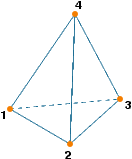
\includegraphics[scale=0.6]{runpylith/figs/tet4}\hspace*{0.5in}%
  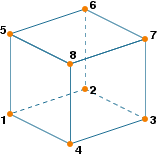
\includegraphics[scale=0.6]{runpylith/figs/hex8}
  \caption{Linear cells available for 3D problems are the tetrahedron (left)
    and the hexahedron (right).}
  \label{fig:3D:cells}
\end{figure}

\subsubsection{\object{Mesh Importer}}

The default mesher component is \object{MeshImporter}, which provides
the capabilities of reading the mesh from files. The \object{MeshImporter} has
several properties and facilities:
\begin{inventory}
  \propertyitem{reorder\_mesh}{Reorder the vertices and cells using the
    reverse Cuthill-McKee algorithm (default is False)}
  \facilityitem{reader}{Reader for a given type of mesh (default is
    \object{MeshIOAscii}).}
  \facilityitem{distributor}{Handles
    distribution of the mesh among processors.}
  \facilityitem{refiner}{Perform global uniform mesh refinement after
    distribution among processors (default is no refinement).}
\end{inventory}
Reordering the mesh so that vertices and cells connected topologically
also reside close together in memory improves overall performance
and can improve solver performance as well.

\userwarning{The coordinate system associated with the mesh must be a
  Cartesian coordinate system, such as a generic Cartesian coordinate
  system or a geographic projection.}

\subsubsection{\object{MeshIOAscii}}

The \object{MeshIOAscii} object is intended for reading small, simple
ASCII files containing a mesh constructed by hand. We use this file
format extensively in the examples. Appendix \vref{sec:format:MeshIOAscii}
describes the format of the files. The properties and facilities of
the \object{MeshIOAscii} object include:
\begin{inventory}
\propertyitem{filename}{Name of the mesh file.}
\facilityitem{coordsys}{Coordinate system associated with the mesh.}
\end{inventory}

\subsubsection{\object{MeshIOCubit}}
\label{sec:MeshIOCubit}

The \object{MeshIOCubit} object reads the NetCDF Exodus II files output from
CUBIT/Trelis. Beginning with CUBIT 11.0, the names of the nodesets are included
in the Exodus II files and PyLith can use these nodeset names or revert
to using the nodeset ids. The properties and facilities associated
with the \object{MeshIOCubit} object are:
\begin{inventory}
\propertyitem{filename}{Name of the Exodus II file.}
\propertyitem{use\_nodeset\_names}{Identify nodesets by name rather than id
(default is True).}
\facilityitem{coordsys}{Coordinate system associated with the mesh.}
\end{inventory}

\subsubsection{\object{MeshIOLagrit}}
\label{sec:MeshIOLagrit}

The \object{MeshIOLagrit} object is used to read ASCII and binary GMV and PSET
files output from LaGriT. PyLith will automatically detect whether
the files are ASCII or binary. We attempt to provide support for experimental
64-bit versions of LaGriT via flags indicating whether the FORTRAN
code is using 32-bit or 64-bit integers. The \object{MeshIOLagrit} properties
and facilities are:
\begin{inventory}
  \propertyitem{filename\_gmv}{Name of GMV file.}
  \propertyitem{filename\_pset}{Name of the PSET file.}
  \propertyitem{flip\_endian}{Flip the endian of values when reading
    binary files (default is False).}
  \propertyitem{io\_int32}{Flag
    indicating that PSET files use 32-bit integers (default is True).}
  \propertyitem{record\_header\_32bt}{Flag indicating FORTRAN record header is
    32-bit (default is True).}
\facilityitem{coordsys}{Coordinate system associated with mesh.}
\end{inventory}

\userwarning{The PyLith developers have not used LaGriT since around 2008
  and the most recent release appears to have been in 2010.}

\subsubsection{\object{Distributor}}

The distributor uses a partitioner to compute which cells should be
placed on each processor, computes the overlap among the processors,
and then distributes the mesh among the processors. The type of
partitioner is set via PETSc settings. The properties and facilities
of the \object{Distributor} include:
\begin{inventory}
\propertyitem{partitioner}{Name of mesh partitioner ['chaco','parmetis'].}
\propertyitem{write\_partition}{Flag indicating that the partition information
should be written to a file (default is False).}
\facilityitem{data\_writer}{Writer for partition information (default
  is \object{DataWriterVTK} for VTK output).}
\end{inventory}
\begin{cfg}[\object{Distributor} parameters in a \filename{cfg} file]
<h>[pylithapp.mesh_generator.distributor]</h>
<p>partitioner</p> = chaco ; Options are 'chaco' (default) and 'parmetis'.
\end{cfg}
METIS/ParMETIS are not included in the PyLith binaries due to licensing
issues. 


\subsubsection{\object{Refiner}}

The refiner is used to decrease node spacing by a power of two by
recursively subdividing each cell by a factor of two. In a 2D triangular
mesh a node is inserted at the midpoint of each edge, splitting each
cell into four cells (see Figure \vref{fig:uniform:refinement:2x}).
In a 2D quadrilateral mesh a node is inserted at the midpoint of each
edge and at the centroid of the cell, splitting each cell into four
cells. In a 3D tetrahedral mesh a node is inserted at the midpoint
of each edge, splitting each cell into eight cells. In a 3D hexahedral
mesh a node is inserted at the midpoint of each edge, the centroid
of each face, and at the centroid of the cell, splitting each cell
into eight cells.

\begin{figure}[htbp]
  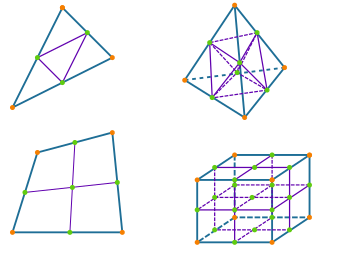
\includegraphics[scale=0.6]{runpylith/figs/refinement2x}
  \caption{Global uniform mesh refinement of 2D and 3D linear
    cells. The blue lines and orange circles identify the edges and
    vertices in the original cells. The purple lines and green circles
    identify the new edges and vertices added to the original cells to
    refine the mesh by a factor of two.}
\label{fig:uniform:refinement:2x}
\end{figure}

Refinement occurs after distribution of the mesh among processors.
This allows one to run much larger simulations by (1) permitting the
mesh generator to construct a mesh with a node spacing larger than
that needed in the simulation and (2) operations performed in serial
during the simulation setup phase, such as, adjusting the topology
to insert cohesive cells and distribution of the mesh among processors
uses this much smaller coarse mesh. For 2D problems the global mesh
refinement increases the maximum problem size by a factor of $4^{n}$,
and for 3D problems it increases the maximum problem size by a factor
of $8^{n}$, where $n$ is the number of recursive refinement levels.
For a tetrahedral mesh, the element quality decreases with refinement
so $n$ should be limited to 1-2.


\subsection{Problem Specification (\protect\facility{problem})}

The problem component specifies the basic parameters of the simulation,
including the physical properties, the boundary conditions, and interface
conditions (faults). The current release of PyLith contains two types
of problems, \object{TimeDependent} for use in static, quasistatic,
and dynamic simulations and \object{GreensFns} for computing static
Green's functions. The general properties facilities include:
\begin{inventory}
  \propertyitem{solver}{Type of solver to use ({\tt linear} or {\tt nonlinear});}
  \facilityitem{solution}{Solution field;}
  \facilityitem{normalizer}{Scales used to nondimensionalize the
    problem (default is \object{NondimElasticQuasistatic});}
  \facilityitem{materials}{Array of materials comprising the domain
    (default is [material]);}
  \facilityitem{bc}{Array of boundary conditions (default is none);}
  \facilityitem{interfaces}{Array of interface conditions, i.e., faults
    (default is none); and}
  \facilityitem{gravity\_field}{Gravity field used to construct body
    forces (default=\object{NullComponent});}
\end{inventory}

\begin{cfg}[Problem parameters in a \filename{cfg} file]
<h>[pylithapp.timedependent]</h>
<p>solver</p> = linear
<f>solution</f> = pylith.problems.SolnDisp
<f>normalizer</f> = spatialdata.units.NondimElasticQuasistatic
<f>materials</f> = [elastic, viscoelastic]
<f>bc</f> = [boundary_east, boundary_bottom, boundary_west]
<f>interfaces</f> = [SanAndreas, SanJacinto]
<f>gravity_field</f> = spatialdata.spatialdb.GravityField
\end{cfg}

The following sections discuss the \facility{solution} and
\facility{normalizer}. Materials, boundary conditions, and interface
conditions are discussed in Chapter \vref{cha:physics} and the gravity
field spatial database is discussed in Section
\vref{sec:gravity:field}.

\subsubsection{Solution Field (\facility{solution})}

The \facility{solution\_field} specifies the subfields of the solution
field along with their discretization. Table
\vref{tab:solution:containers} shows predefined containers for common
subfield collections. Users can create their own containers if they
add different material formulations.

\important{The order of the subfields within the solution field must
  be consistent between the \object{Solution} field object and the
  point-wise functions. The predefined containers are setup to help
  ensure that this is true.}

\important{When a Lagrange multiplier for fault interfaces is
  included, it should always be the last solution subfield. It is
  special case, because it is discretization only on the cohesive
  cells and not over the entire domain.}

\begin{table}[htbp]
  \caption{Predefined containers for solution subfields.}
  \label{tab:solution:containers}
  \begin{tabular}{lll}
    \toprule
    \thead{Object} & \thead{Subfields} & \thead{Use Cases} \\
    \midrule
    \object{SolnDisp} & displacement & Elasticity w/o inertia and faults \\
    \object{SolnDispVel} & displacement, velocity & Elasticity w/inertia and w/o faults \\
    \object{SolnDispLagrange} & displacement, lagrange\_fault & Elasticity w/faults \\
    \object{SolnDispVelLagrange} & displacement, lagrange\_fault & Elasticity w/faults \\
    \object{SolnDispPres} & displacement, pressure & Incompressible elasticity w/o faults \\
    \object{SolnDispPresLagrange} & displacement, pressure, lagrange\_fault & Incompressible elasticity w/o faults \\
    \bottomrule
  \end{tabular}
\end{table}

Each subfield is a \object{SolutionSubfield} object with the following properties:
\begin{inventory}
  \propertyitem{alias}{User-specified name for subfield to use in
    output (default is the PyLith-specified name);}
  \propertyitem{basis\_order}{Order for basis functions (default=1);}
  \propertyitem{quadrature\_order}{Order of quadrature to use in
    integration (default=1);}
  \propertyitem{dimension}{Topological dimension
    associated with subfield (default=-1 and should not be
    changed); and}
  \propertyitem{finite\_element\_space}{Finite-element space ({\tt
      polynomial} or {\tt point; defaults=polynomial}). Point space corresponds to delta
    functions at the quadrature points;}
\end{inventory}

\begin{cfg}[Setting discretization information for a \object{SolnDispLagrange} component in a \filename{cfg} file]
<h>[pylithapp.problem]</h>
<f>solution</f> = pylith.problems.SolnDispLagrange

<h>[pylithapp.problem.solution.subfields]</h>
<p>displacement.basis_order</p> = 1
<p>displacement.quadrature_order</p> = 1

<p>lagrange_fault.basis_order</p> = 1
<p>lagrange_fault.quadrature_order</p> = 1
\end{cfg}


\subsubsection{Nondimensionalization (\facility{normalizer})}

PyLith rescales all parameters provided by the user so that the
simulation solves the equations using nondimensional quantities.  This
permits application of PyLith to problems across a vast range of
spatial and temporal scales. The scales used to nondimensionalize the
problem are length, pressure, density, and time. PyLith provides two
normalizer objects to make it easy to provide reasonable scales for
the nondimensionalization. The \object{NondimElasticQuasistatic}
normalizer (which is the default) has the following properties:
\begin{inventory}
  \propertyitem{length\_scale}{Distance to nondimensionalize length
    (default is 1.0 km).}
  \propertyitem{shear\_modulus}{Shear modulus to nondimensionalize
    pressure (default is 3.0e+10 Pa).}
  \propertyitem{relaxation\_time}{Relaxation time to
    nondimensionalize time (default is 1.0 year).}
\end{inventory}
\begin{cfg}[\object{NondimElasticQuasistatic} parameters in a \filename{cfg} file]
<h>[pylithapp.timedependent.normalizer]</h>
<p>length_scale</p> = 1.0*km
<p>shear_modulus</p> = 3.0e+10*Pa
<p>relaxation_time</p> = 1.0*yr
\end{cfg}
The \object{NondimElasticDynamic} normalizer has the following
properties:
\begin{inventory}
  \propertyitem{shear\_wave\_speed}{Shear wave speed used to
    nondimensionalize length and pressure (default is 3.0 km/s).}
  \propertyitem{mass\_density}{Mass density to nondimensionalize
    density and pressure (default is 3.0e+3 kg/m$^{3}$).}
  \propertyitem{wave\_period}{Period of seismic waves used to
    nondimensionalize time (default is 1.0 s).}
\end{inventory}
\begin{cfg}[\object{NondimElasticDynamic} parameters in a \filename{cfg} file]
<h>[pylithapp.timedependent.normalizer]</h>
<p>shear_wave_speed</p> = 3.0*km/s
<p>mass_density</p> = 3.0e+3*kg/m**3
<p>wave_period</p> = 1.0*s
\end{cfg}

\important{The default nondimensionalization is reasonable for many
  problems; however, it may be necessary to change the default values
  in some cases. When doing this, keep in mind that the
  nondimensionalization generally applies to the minimum values
  encountered for a problem.  For example, in a quasistatic problem,
  the \property{length\_scale} should be on the order of the minimum
  cell size. Similarly, the \property{relaxation\_time} should be on
  the order of the minimum relaxation time or time scale associated
  with time-dependent boundary and interface conditions.}


\subsubsection{Solution Observers (\facility{solution\_observers})}
\label{sec:solution:observers}

The solution observers get notified of updates to the solution. Table
\vref{solution:observers} lists the current implementations of
solution observers, which are used for output.

\begin{table}[htbp]
  \caption{Solution observers.}
  \label{tab:solution:observers}
  \begin{tabular}{lll}
    \toprule
    \thead{Object} & \thead{Use Cases} \\
    \midrule
    \object{OutputSoln} & Output of the solution over the domain; \\
    \object{OutputSolnBoundary} & Output of the solution over an external boundary \\
    \object{OutputSolnPoints} & Output of the solution at discrete points \\
    \bottomrule
  \end{tabular}
\end{table}

All of the solution observers have the following properties:
\begin{inventory}
  \propertyitem{data\_fields}{List of solution subfields to observer/output (default=all which will output all of the subfields);}
  \facilityitem{writer}{Writer for data (default=\object{DataWriterHDF5});}
  \facilityitem{trigger}{Trigger defining how often output is written (default=\object{OutputTriggerStep}); and}
  \facilityitem{output\_basis\_order}{Basis order for output of
    fields. Valid values are 0 and 1 (default=1).}
\end{inventory}
Fields with a basis order of 0 are kept at a basis order of 0 when output.
Fields with a basis order of 1 are written as vertex fields, whereas fields with a basis order of 0 are written as cell fields.

\object{OutputSolnBoundary} adds a property:
\begin{inventory}
  \propertyitem{label}{Label (name of nodeset/pset) identifier of boundary (required);}
\end{inventory}
See Section \vref{sec:output} for detailed information about the
available components for the \facility{writer} and \facility{trigger} facilities.

\begin{cfg}[Setting \object{OutputSolnBoundary} parameters in a \filename{cfg} file]
<h>[pylithapp.problem.solution_observers.boundary]</h>
<p>label</p> = boundary_groundsurf
<p>writer.filename</p> = output/step01-grounssurf.h5
\end{cfg}

\paragraph{Output at Arbitrary Points (\protect\object{OutputSolnPoints})}
\label{sec:output:points}

In many situations with recorded observations, one would like to
extract the solution at the same locations as the recorded
observation. Rather than forcing the finite-element discretization to
be consistent with the observation points, PyLith includes a
specialized solution observer, \object{OutputSolnPoints}, to interpolate
the solution to arbitrary points. The locations
are specified in a text file. The \object{OutputSolnPoints}
includes:
\begin{inventory}
  \propertyitem{data\_fields}{List of solution subfields to
    observer/output (default=all which will output all of the
    subfields);}
  \facilityitem{reader}{Reader for points list (default
    is \object{PointsList}); and}
\end{inventory}

\subsubsection{\object{PointsList} Reader}

This object corresponds to a simple text file containing a list of
points (one per line) where output is desired. See \vref{sec:format:PointsList}
for file format specifications. The points are specified in the coordinate
system specified by \object{OutputSolnPoints}. The coordinates will be transformed
into the coordinate system of the mesh prior to interpolation. The
properties available to customize the behavior of \object{PointsList}
are:
\begin{inventory}
\propertyitem{filename}{Names of file containing list of points.}
\propertyitem{comment\_delimiter}{Delimiter at beginning of line to identify
comments (default is \#).}
\propertyitem{value\_delimiter}{Delimiter used to separate values (default is
whitespace).}
\end{inventory}



\subsection{PETSc Settings (\protect\facility{petsc})}
\label{sec:petsc:options}

PyLith relies on PETSc for the finite-element data structures, linear
and nonlinear solvers, and time-stepping algorithms. PETSc has its own
object-oriented interface for specifying runtime options. Instead of
trying to maintain a Pyre interface to all of the PETSc options, we
use a single \facility{petsc} facility to collect all of the PETSc
options and pass them to PETSc.

PETSc time-stepping options are discussed in Section
\vref{sec:problems:timedependent}.

\subsubsection{Monitor/Logging Settings}

Table \vref{tab:pesc:options:monitor} shows the main monitoring
options offered by PETSc. Our recommended settings for all simulations
include:
\begin{cfg}[Recommended PETSc monitoring settings as set in a \filename{cfg} file.]
<h>[pylithapp.petsc]</h>
# Trigger errors if linear or nonlinear solver fails to converge.
<p>ksp_error_if_not_converged</p> = true
<p>snes_error_if_not_converged</p> = true

# Monitor converged reasons
<p>ksp_converged_reason</p> = true
<p>snes_converged_reason</p> = true

# Monitor time-stepping and nonlinear solver
<p>ts_monitor</p> = true
<p>snes_monitor</p> = true
<p>snes_linesearch_monitor</p> = true
\end{cfg}
When optimizing and troubleshooting solver settings, we usually turn on all the monitoring.

\begin{table}[htbp]
  \caption{Description of PETSc monitoring settings.}
  \label{tab:petsc:options:monitor}
  \begin{tabular}{lp{4.0in}}
    \toprule
    \thead{Option} & \thead{Description} \\
    \midrule
% log
    \property{log\_view} & Show logging objects and events. \\

% TS
    \property{ts\_monitor} & Show time-stepping progress. \\
% KSP
    \property{ksp\_monitor} & Show preconditioned residual norm. \\
    \property{ksp\_view} & Show linear solver parameters. \\
    \property{ksp\_error\_if\_not\_converged} & Generate an error if linear solver does not converge. \\
    \property{ksp\_converged\_reason} & Indicate why iterating stopped in linear solve. \\
% SNES
    \property{snes\_monitor} & Show residual norm for each nonlinear solve iteration. \\
    \property{snes\_view} & Show nonlinear solver parameters. \\
    \property{snes\_error\_if\_not\_converged} & Generate an error if nonlinear solver does not converge. \\
    \property{snes\_converged\_reason} & Indicate why iterating stopped in nonlinear solve. \\
    \property{snes\_linesearch\_monitor} & Show line search information in nonlinear solve. \\
    \bottomrule 
  \end{tabular}
\end{table}


\subsubsection{Solver Settings}

For most problems we use the GMRES method from Saad and Schultz for
the linear solver with solver tolerances around 1.0e-10. When running
large problems, we often raise the solver tolerances by one or two
orders of magnitude to reduce runtime while still achieving suitable
accuracy.

See
\href{http://www.mcs.anl.gov/petsc/petsc-as/documentation/linearsolvertable.html}{PETSc
  linear solver table} for a list of PETSc options for linear solvers
and preconditioners.

\usertip{It is important to keep in mind the resolution of the model and
  observations when setting solver tolerances. For example, matching
  observations with an accuracy of 1.0\si{\milli\meter} does not
  require solving the equations to an accuracy of
  0.0001\si{\milli\meter}.}


\begin{table}[htbp]
  \caption{Recommended starting point for PETSc solver tolerances.}
  \label{tab:petsc:options:solver}
  \begin{tabular}{lcp{4.5in}}
    \toprule
    \thead{Property} & \thead{Value} & \thead{Description} \\
    \midrule
% KSP
    \property{ksp\_rtol} & 1.0e-10 & Stop iterating when the preconditioned KSP residual norm has this amount relative to its starting value.\\
    \property{ksp\_atol} & 1.0e-12 & Stop iterating when the preconditioned KSP residual normal is smaller than this value.\\
% SNES
    \property{snes\_rtol} & 1.0e-10 & Stop iterating when the SNES residual norm has this amount relative to its starting value.\\
    \property{snes\_atol} & 1.0e-10 & Stop iterating when the SNES residual normal is smaller than this value.\\
    \bottomrule 
  \end{tabular}
\end{table}

\paragraph{Settings for small problems}

When running small test problems (about 1k or less unknowns) it is very
handy to use a robust preconditioner so that issues related to the boundary
conditions, material parameters, etc. are more obvious. We recommend
using Incomplete (ILU) factorization.

\begin{cfg}[Recommended PETSc solver settings for small problems]
<h>[pylithapp.petsc]</h>
<p>pc_type</p> = ilu
<p>ksp_type</p> = gmres
\end{cfg}

\paragraph{Settings for medium problems}

When running slightly larger problems (about 10k or less unknowns),
the Additive Schwarz Method (ASM) using Incomplete LU (ILU)
factorization preconditioner is usually more efficient.

\begin{cfg}[Recommended PETSc solver settings for medium problems]
<h>[pylithapp.petsc]</h>
<p>pc_type</p> = asm
<p>ksp_type</p> = gmres
\end{cfg}

\paragraph{Efficient settings for elasticity without a fault}

Algebraic multigrid preconditioner usually works very well on
elasticity problems.

\begin{cfg}[Recommended PETSc solver settings for solving elasticity problems without a fault]
<h>[pylithapp.petsc]</h>
<p>pc_type</p> = ml
<p>ksp_type</p> = gmres
\end{cfg}

\important{The ML algebraic multigrid preconditioner is only available
  if you build PETSc with the ML package. These features are included
  in the PyLith binary packages.}

\paragraph{Efficient settings for elasticity with a fault}

The Lagrange multiplier solution subfield introduces a saddle point in
the system of equations, so we use a Schur complement approach. These
settings are available in
\filename{\$PYLITH\_DIR/share/settings/solver\_fault\_exact.cfg}.

\begin{cfg}[Recommended PETSc solver settings for solving elasticity problems with a fault]
<h>[pylithapp.petsc]</h>
<p>pc_type</p> = fieldsplit
<p>pc_use_amat</p> = true
<p>pc_fieldsplit_type</p> = schur
<p>pc_fieldsplit_schur_factorization_type</p> = full
<p>pc_fieldsplit_dm_splits</p> = true
<p>fieldsplit_displacement_ksp_type</p> = preonly
<p>fieldsplit_displacement_pc_type</p> = lu
<p>fieldsplit_lagrange_multiplier_fault_pc_type</p> = jacobi
<p>fieldsplit_lagrange_multiplier_fault_ksp_type</p> = gmres
<p>fieldsplit_lagrange_multiplier_fault_ksp_rtol</p> = 1.0e-11
<p>fieldsplit_lagrange_multiplier_fault_ksp_converged_reason</p> = true
\end{cfg}


\userwarning{The split fields and algebraic multigrid preconditioning
  currently fails in problems with a nonzero null space. This most
  often occurs when a problem contains multiple faults that extend
  through the entire domain and create subdomains without any
  Dirichlet boundary conditions. The current workaround is to use the
  Additive Schwarz preconditioner without split fields.  See Section
  \vref{sec:Troubleshooting} for the error message encountered in this
  situation.}

\paragraph{Efficient settings for incompressible elasticity}

The pressure solution subfield introduces a saddle point in the system
of equations, so we again use a Schur complement approach. This time
we can use algebraic multigrid preconditioning on each block. These
settings are available in
\filename{\$PYLITH\_DIR/share/settings/solver\_incompressible\_elasticity.cfg}.

\begin{cfg}[Recommended PETSc solver settings for solving incompressible elasticity problems without a fault]
<h>[pylithapp.petsc]</h>
<p>pc_type</p> = fieldsplit
<p>pc_fieldsplit_type</p> = schur
<p>pc_fieldsplit_schur_fact_type</p> = full
<p>pc_fieldsplit_schur_precondition</p> = full
<p>fieldsplit_displacement_pc_type</p> = lu
<p>fieldsplit_pressure_pc_type</p> = lu
\end{cfg}


% End of file

\input{./runpylith/problems.tex}
\input{./runpylith/databases.tex}
\input{./runpylith/labels.tex}
\section{Output}

PyLith currently supports output to HDF5/Xdmf and VTK files, which can
be imported directly into a number of visualization tools, such as
ParaView, Visit, and MayaVi. The HDF5 files can also be directly
accessed via Matlab and Python modules, such as h5py and
PyTables. PyLith v3.x supports output of the solution subfields (see
Section \vref{sec:solution:observers}) all auxiliary fields
(material properties, boundary condition parameters, and fault interface
parameters, etc.) and fields derived from the auxiliary field and/or
solution, such as stress and stress.

HDF5 writer provides parallel binary output, whereas the VTK writer
provides serial ASCII output. Additionally, with the VTK writer each
time step is written to a separate file; the HDF5 writer puts all
information for a given domain, boundary condition, or fault interface
into a single file.


\subsection{Physics Observer (\object{OutputPhysics})}

Analogous to the \object{OutputSoln} objects discussed in Section
\vref{sec:solution:observers} for output of the solution, the physics
objects (material, boundary conditions, and fault interfaces) have
\object{OutputPhysics} objects to provide output of the solution,
properties, state variables, etc. 

The parameters for the \object{OutputPhysics} are:
\begin{inventory}
  \propertyitem{info\_fields}{List of auxiliary subfields to observer/output (default=all which will output all of the subfields);}
  \propertyitem{data\_fields}{List of solution subfields to observer/output (default=all which will output all of the subfields);}
  \facilityitem{writer}{Writer for data (default=\object{DataWriterHDF5});}
  \facilityitem{trigger}{Trigger defining how often output is written (default=\object{OutputTriggerStep}); and}
  \facilityitem{field\_filter}{Filter for output fields (default=\object{FieldFilterNone}).}
\end{inventory}

\begin{cfg}[\object{PhysicsOutput} parameters in a \filename{cfg} file]
<h>[pylithapp.problem.materials.elastic.observers.observer]</h>
<p>writer.filename</p> = output/step01-elastic.h5
<f>field_filter</f> = pylith.meshio.FieldFilterNone
\end{cfg}

\subsection{Output Field Filter (\facility{field\_filter})}

Sometimes fields may not be in the form a user wants. For example, the
displacement solution subfield may have a basis order of 2 with
degrees of freedom associated with edges, which is incompatible with
most visualization packages that require information be provided with
a basis order of 1 (vertex data) or 0 (cell data). The
\facility{field\_filter} facility of the \object{OutputPhysics} object
allows passing a field through a ``filter'' to yield the desired form
of the output. The default filter is \object{FieldFilterNone}, which
simply passes the input field on to the \facility{writer} for
output. The \object{FieldFilterProject} object provides the ability to
project the input field to a lower basis order.

\subsubsection{Projecting to lower basis order (\object{FieldFilterProject})}

This filter projects a field to a lower basis order. It is most often
used to reduce the basis order of solution subfields, e.g,,
displacement, to a basis order of 1 from a basis order of 2, so that
the solutino field can be visualized in common ParaView, etc.
The \object{fieldFilterProject} property is:
\begin{inventory}
  \propertyitem{basis\_order}{Basis order of the projected field (default=1).}
\end{inventory}

\begin{cfg}[Using \object{FieldFilterProject} with solution output in
  a \filename{cfg} file]
<h>[pylithapp.problem.solution_observers.domain]</h>
<p>writer.filename</p> = output/step01-domain.h5
<f>field_filter</f> = pylith.meshio.FieldFilterProject
<p>field_filter.basis_oder</p> = 0
\end{cfg}


\subsection{Data Writers (\facility{writer})}

\subsubsection{VTK Output (\object{DataWriterVTK})}

PyLith writes legacy (non-XML) VTK files. These are simple files with
vertex coordinates, the mesh topology, and fields over vertices and/or
cells. Each time step is written to a different file. The time stamp
is included in the filename with the decimal point removed. This allows
automatic generation of animations with many visualization packages
that use VTK files. The default time stamp is the time in seconds,
but this can be changed using the normalization constant to give a
time stamp in years, tens of years, or any other value.


The parameters for the VTK writer are:
\begin{inventory}
\propertyitem{filename}{Name of VTK file.}
\propertyitem{time\_format}{C-style format string for time stamp in filename.
The decimal point in the time stamp will be removed for compatibility
with VTK visualization packages that provide seamless animation of
data from multiple VTK files.}
\propertyitem{time\_constant}{Value used to normalize time stamp in VTK files
(default is 1.0 s).}
\end{inventory}

\userwarning{We strongly discourage use of using VTK output. It is slow,
  inefficient, and not easily read from post-processing scripts. We
  strongly recommwnd using HDF5 output instead, which is the default
  starting in PyLith v3.0.0.}

\subsubsection{HDF5/Xdmf Output (\object{DataWriterHDF5}, \object{DataWriterHDF5Ext})}
\label{sub:HDF5/Xdmf-Output}

HDF5 files provide a flexible framework for storing simulation data
with datasets in groups logically organized in a tree structure analogous
to files in directories. HDF5 output offers parallel, multi-dimensional
array output in binary files, so it is much faster and more convenient
than the VTK output which uses ASCII files and separate files for
each time step. Standards for organizing datasets and groups in HDF5
files do not exist for general finite-element software in geodynamics.
Consequently, PyLith uses its own simple layout show in Figure \vref{fig:hdf5:layout}.
In order for visualization tools, such as ParaView, to determine which
datasets to read and where to find them in the hierarchy of groups
within the HDF5 file, we create an Xdmf (eXtensible Data Model and
Format, \url{www.xdmf.org}) metadata file that provides this information.
This file is written when PyLith closes the HDF5 file at the end of
the simulation. In order to visualize the datasets in an HDF5 file,
one simply opens the corresponding Xdmf file (the extension is \filename{xmf})
in ParaView or Visit. The Xdmf file contains the relative path to
the HDF5 file so the files can be moved but must be located together
in the same directory. 

\important{The Xdmf format supports
representation of two- and three-dimensional coordinates of points,
scalar fields, and three-dimensional vector and tensor fields but
not two-dimensional vector or tensor fields. Consequently, for two-dimensional
vector fields we build a three-component vector from the two-component
vector (x and y components) and a separate zero scalar field (z component).
For tensor fields, we create a scalar field for each of the tensor
components, adding the component as a suffix to the name of the field.}

\begin{figure}[htbp]
  \includegraphics{runpylith/figs/hdf5layout}
  \caption{General layout of a PyLith HDF5 file. The orange rectangles
    with rounded corners identify the groups and the blue rectangles
    with sharp corners identify the datasets. The dimensions of the
    data sets are shown in parentheses. Most HDF5 files will contain
    either \texttt{vertex\_fields} or \texttt{cell\_fields} but not
    both.}
 \label{fig:hdf5:layout}
\end{figure}

See Table \vref{tab:materials:statevars} in Section
\vref{sec:material:parameters} for a table of component values for
tensor output in HDF5 files. To avoid confusion about the ordering of
components for tensor data, we separate the components in the Xdmf
file.

The \object{DataWriterHDF5} and \object{DataWriterHDF5Ext} property is:
\begin{inventory}
  \propertyitem{filename}{Name of HDF5 file (default=output.h5; the
    Xdmf filename is generated from the same prefix).}
\end{inventory}

\begin{cfg}[\object{DataWriterHDF5Ext} parameters in a \filename{cfg} file]
<h>[pylithapp.timedependent.domain.output]</h>
<p>output_freq</p> = time_step
<p>time_step</p> = 1.0*yr
<p>cell_data_fields</p> = [displacement, velocity]
<f>writer</f> = pylith.meshio.DataWriterHDF5Ext
<p>writer.filename</p> = dislocation.h5
\end{cfg}
In this example, we change the writer from the default VTK writer to
the HDF5 writer with external datasets (\object{DataWriterHDF5Ext})
for output over the domain.

HDF5 files do not contain self-correcting features that allow a file
to be read if part of a dataset is corrupted. This type of error can
occur if a job terminates abnormally in the middle or at the end of a
simulation on a large cluster or other parallel machine. Fortunately,
HDF5 also offers the ability to store datasets in external binary
files with the locations specified by links in the HDF5 file. Note
that the use of external data files results in one data file per
dataset in addition to the HDF5 and Xdmf files. The external data
files use the name of the HDF5 file with the dataset name added to the
prefix and the \filename{h5} suffix replaced by \filename{dat}. The
HDF5 files include relative paths to the external data files, so these
files can also be moved, but they, too, must be kept together in the
same directory. This provides a more robust method of output because
one can generate an HDF5 file associated with the uncorrupted portions
of the external data files should an error occur. Currently, PyLith
does not include a utility to do this, but we plan to add one in a
future release. Thus, there are two options when writing PyLith output
to HDF5 files: (1) including the datasets directly in the HDF5 files
themselves using the \object{DataWriterHDF5} object or (2) storing the
datasets in external binary files with just metadata in the HDF5 files
using the \object{DataWriterHDF5Ext} object. Both methods provide
similar performance because they will use MPI I/O if it is available.

\userwarning{Storing the datasets within the HDF5 file in a parallel
  simulation requires that the HDF5 library be configured with the
  \commandline{-{}-enable-parallel} option. The binary PyLith packages
  include this feature and it is a default setting in building HDF5
  via the PyLith Installer.}

Accessing the datasets for additional analysis or visualization is
nearly identical in the two methods because the use of external data
files is completely transparent to the user except for the presence
of the additional files. Note that in order for ParaView to find the
HDF5 and external data files, it must be run from the same relative
location where the simulation was run. For example, if the simulation
was run from a directory called ``work'' and the HDF5/Xdmf files
were written to ``work/output'', then ParaView should be run from
the ``work'' directory. See Table \vref{tab:materials:statevars}
in Section \vref{sec:material:parameters} for a table of component
values for tensor output.

\begin{cfg}[Selecting \object{DataWriterHDF5Ext} in a \filename{cfg}
  file]
<h>[pylithapp.problem]</h>
<f>solution_observers</f> = [domain]
<f>solution_observers.domain>/f> = pylith.mehsio.DataWriterHDF5Ext

<h>[pylithapp.problem.solution_observers.domain]</h>
<p>writer.filename</p> = output/step01-domain.h5
\end{cfg}

\subsubsection{HDF5 Utilities}

HDF5 includes several utilities for examining the contents of HDF5
files. \filename{h5dump} is very handy for dumping the hierarchy,
dimensions of datasets, attributes, and even the dataset values to
stdout. 
\begin{shell}
# Dump the entire HDF5 file (not useful for large files).
$ h5dump mydata.h5

# Dump the hierarchy of an HDF5 file.
$ h5dump -n mydata.h5

# Dump the hierarchy with dataset dimensions and attributes.
$ h5dump -H mydata.h5

# Dump dataset 'vertices' in group '/geometry' to stdout.
$ h5dump -d /geometry/vertices mydata.h5
\end{shell}
We have also include a utility \filename{pylith\_genxdmf} (see Section
\vref{sec:pylith:genxdmf}) that generates an appropriate Xdmf file
from a PyLith HDF5 file. This is very useful if you add fields to
HDF5 files in post-processing and wish to view the results in ParaView
or Visit.


\subsection{Output Triggers (\facility{trigger})}
\newfeature{3.0.0}

By default PyLith will write the requested output after every time
step. In many cases we prefer to save the solution, state variables,
etc at a coarser temporal resolution. The \object{OutputTriggerStep}
controls the decimation of the output by time step, and the
\object{OutputTriggerTime} controls the decimation of the output via
time. For uniform time stepping these are equivalent.

\subsubsection{Decimate by time step (\object{OutputTriggerStep})}

\object{OutputTriggerStep} decimates the output by skipping a
user-specified number of time steps. The property is
\begin{inventory}
  \propertyitem{num\_skip}{Number of solution steps to skip between
    writes (default=0).}
\end{inventory}

  
\subsubsection{Decimate by time (\object{OutputTriggerTime})}

\object{OutputTriggerTime} decimates the output by skipping a
user-specified elasped time. The property is
\begin{inventory}
  \propertyitem{elapsed\_time}{Elasped time between writes (default=0.0*s).}
\end{inventory}
 
\usertip{Due to roundoff error in determining the simulation time over
  many time steps, a simulation may occasionally skip writing output
  unexpectedly when using \object{OutputTriggerTime}. The best
  workaround is to use an \property{elapsed\_time} that is a fraction
  of the time step size smaller than the desired elapsed time, such as
  0.9999*year instead of 1.0*year.}
  
% End of file

\section{Utilities}
\label{sec:runpylith:utilities}

The PyLith distribution contains several utilities for working with PyLith simulations and processing output.
These Python scripts are all installed into the same \filename{bin} directory as the \filename{pylith} application with the exception of the \filename{pyre\_doc.py} script which is installed as part of Pythia/Pyre.

\begin{description}
  \item[\filename{pyre\_doc}] Display the Pyre properties and facilities available for a given component.
  \item[\filename{pylith\_cfgsearch}] Search and display metadata in \filename{.cfg} files.
  \item[\filename{pylith\_runner}] Run all PyLith simulations in a given path.
  \item[\filename{pylith\_eqinfo}] Compute earthquake rupture metrics from PyLith output.
  \item[\filename{pylith\_genxdmf}] Generate Xdmf files from HDF5 files written by PyLith.
\end{description}
  
\subsection{\filename{pyre\_doc.py}}
\newfeature{v3.0.0}

This utility is part of the Pythia/Pyre framework.
It will be installed to the \filename{bin} directory where Pythia/Pyre is installed.
This utility extracts the Python docstrings and help information for Pyre components.

\warning{This utility does not work on the PyLithApp application object because it is a mpi.Application object.}

\begin{shell}
pyre_doc.py [--help] [--short] OBJECT
\end{shell}

\begin{description}
\item[\commandline{-{}-help}] Display help information for script.
\item[\commandline{-{}-short}] Display only the docstrings for the specified module or object. The default is to display the information for the specified object and all child objects, such as classes within a module.
\item[OBJECT] Full path to Python module or object, such as \filename{pylith.problems.Problem} (module) or \filename{pylith.problems.Problem.Problem} (object).
\end{description}

\begin{shell}[Example of running \filename{pyre\_doc.py} on \filename{pylith.problems.Problem}]
$ pyre_doc.py pylith.problems.Problem
No help available for module pylith.problems.Problem.

class Problem
Python abstract base class for crustal dynamics problems.

    FACTORY: problem

facilities of 'problem':
    bc=<component name>: Boundary conditions.
        current value: 'emptybin', from {default}
        configurable as: emptybin, bc
    defaults=<component name>: Default options for problem.
        current value: 'problem_defaults', from {default}
        configurable as: problem_defaults, defaults
    gravity_field=<component name>: Database used for gravity field.
        current value: 'nullcomponent', from {default}
        configurable as: nullcomponent, gravity_field
    interfaces=<component name>: Interior surfaces with constraints or constitutive models.
        current value: 'emptybin', from {default}
        configurable as: emptybin, interfaces
    materials=<component name>: Materials in problem.
        current value: 'homogeneous', from {default}
        configurable as: homogeneous, materials
    normalizer=<component name>: Nondimensionalizer for problem.
        current value: 'nondimelasticquasistatic', from {default}
        configurable as: nondimelasticquasistatic, normalizer
    solution=<component name>: Solution field for problem.
        current value: 'solution', from {default}
        configurable as: solution
    solution_observers=<component name>: Observers (e.g., output) for solution.
        current value: 'singlesolnobserver', from {default}
        configurable as: singlesolnobserver, solution_observers
properties of 'problem':
    formulation=<str>: Formulation for equations.
        default value: 'quasistatic'
        current value: 'quasistatic', from {default}
        validator: (in ['quasistatic', 'dynamic', 'dynamic_imex'])
    help=<bool>: prints a screen that describes my traits
        default value: False
        current value: False, from {default}
    help-components=<bool>: prints a screen that describes my subcomponents
        default value: False
        current value: False, from {default}
    help-persistence=<bool>: prints a screen that describes my persistent store
        default value: False
        current value: False, from {default}
    help-properties=<bool>: prints a screen that describes my properties
        default value: False
        current value: False, from {default}
    solver=<str>: Type of solver to use ['linear', 'nonlinear'].
        default value: 'linear'
        current value: 'linear', from {default}
        validator: (in ['linear', 'nonlinear'])
\end{shell}
      
\subsection{\filename{pylith\_cfgsearch}}
\newfeature{v3.0.0}

This utility searches and displays the metadata in \filename{.cfg} files based on criteria provided via the command line.

\begin{shell}
pylith_cfgsearch [--help] [--path SEARCHPATH] [--display DISPLAY] [--verbose] [--keywords KEYWORDS]
    [--features FEATURES] [--authors AUTHORS] [--version VERSION] [--incompatible]
\end{shell}

\begin{description}
\item[-{}-help] DIsplay help information for script.
\item[-{}-path SEARCHPATH] Search path for .cfg files (default: .).
\item[-{}-display DISPLAY] List of metadata to display in search results (default: all).
\item[-{}-keywords KEYWORDS] Comma delimited list of keywords for filtering search results (default: None).
\item[-{}-features FEATURES] Comma delimited list of features for filtering search results (default: None).
\item[-{}-authors AUTHORS] Comma delimited list of authors for filtering search results (default: None).
\item[-{}-version VERSION] PyLith version for filtering search results (default: None).
\item[-{}-verbose] Report missing metadata (default: False).
\item[-{}-incompatible] Filter search results to show incompatible parameter files (default: False).
\end{description}

\begin{shell}[Example of running \filename{pylith\_cfgsearch} in \filename{examples/2d/strikeslip}.]
$ pylith_cfgsearch
step01_slip.cfg v1.0.0; requires PyLith >=3.0 and <4.0
    Coseismic prescribed slip with zero displacement Dirichlet boundary conditions.
    Authors: Brad Aagaard
    Keywords: example, 2D, strike slip, prescribed slip
    Features:
        Triangular cells, pylith.meshio.MeshIOCubit, pylith.problems.TimeDependent, pylith.materials.Elasticity,
        pylith.materials.IsotropicLinearElasticity, pylith.faults.FaultCohesiveKin, pylith.faults.KinSrcStep, field split
        preconditioner, Schur complement preconditioner, pylith.bc.DirichletTimeDependent, spatialdata.spatialdb.UniformDB,
        pylith.meshio.OutputSolnBoundary, pylith.meshio.DataWriterHDF5, Static simulation
    pylith step01_slip.cfg
step02_slip_velbc.cfg v1.0.0; requires PyLith >=3.0 and <4.0
    Coseismic prescribed slip with velocity Dirichlet boundary conditions.
    Authors: Brad Aagaard
    Keywords: example, 2D, strike slip, prescribed slip, velocity boundary conditions
    Features:
        Triangular cells, pylith.meshio.MeshIOCubit, pylith.problems.TimeDependent, pylith.materials.Elasticity,
        pylith.materials.IsotropicLinearElasticity, pylith.faults.FaultCohesiveKin, pylith.faults.KinSrcStep, field split
        preconditioner, Schur complement preconditioner, pylith.bc.DirichletTimeDependent, spatialdata.spatialdb.UniformDB,
        pylith.meshio.OutputSolnBoundary, pylith.meshio.DataWriterHDF5, Quasistatic simulation, spatialdata.spatialdb.SimpleDB
    pylith step02_slip_velbc.cfg
step03_multislip_velbc.cfg v1.0.0; requires PyLith >=3.0 and <4.0
    Coseismic prescribed slip with multiple ruptures and velocity Dirichlet boundary conditions.
    Authors: Brad Aagaard
    Keywords: example, 2D, strike slip, prescribed slip, multiple fault ruptures, velocity boundary conditions
    Features:
        Triangular cells, pylith.meshio.MeshIOCubit, pylith.problems.TimeDependent, pylith.materials.Elasticity,
        pylith.materials.IsotropicLinearElasticity, pylith.faults.FaultCohesiveKin, pylith.faults.KinSrcStep, field split
        preconditioner, Schur complement preconditioner, pylith.bc.DirichletTimeDependent, spatialdata.spatialdb.UniformDB,
        pylith.meshio.OutputSolnBoundary, pylith.meshio.DataWriterHDF5, Quasistatic simulation, spatialdata.spatialdb.SimpleDB
    pylith step03_multislip_velbc.cfg
\end{shell}

\begin{shell}[Example of running \filename{pylith\_cfgsearch} in \filename{examples/2d/strikeslip}, limiting output to the description and keywords.]
$ pylith_cfgsearch --display=description,keywords
step01_slip.cfg
    Coseismic prescribed slip with zero displacement Dirichlet boundary conditions.
    Keywords: example, 2D, strike slip, prescribed slip
step02_slip_velbc.cfg
    Coseismic prescribed slip with velocity Dirichlet boundary conditions.
    Keywords: example, 2D, strike slip, prescribed slip, velocity boundary conditions
step03_multislip_velbc.cfg
    Coseismic prescribed slip with multiple ruptures and velocity Dirichlet boundary conditions.
    Keywords: example, 2D, strike slip, prescribed slip, multiple fault ruptures, velocity boundary conditions
\end{shell}

\begin{shell}[Example of running \filename{pylith\_cfgsearch} in \filename{examples/2d/strikeslip}, filtering search results to quasistatic simulations.]
$ pylith_cfgsearch --features="Quasistatic simulation"
step02_slip_velbc.cfg v1.0.0; requires PyLith >=3.0 and <4.0
    Coseismic prescribed slip with velocity Dirichlet boundary conditions.
    Authors: Brad Aagaard
    Keywords: example, 2D, strike slip, prescribed slip, velocity boundary conditions
    Features:
        Triangular cells, pylith.meshio.MeshIOCubit, pylith.problems.TimeDependent, pylith.materials.Elasticity,
        pylith.materials.IsotropicLinearElasticity, pylith.faults.FaultCohesiveKin, pylith.faults.KinSrcStep, field split
        preconditioner, Schur complement preconditioner, pylith.bc.DirichletTimeDependent, spatialdata.spatialdb.UniformDB,
        pylith.meshio.OutputSolnBoundary, pylith.meshio.DataWriterHDF5, Quasistatic simulation, spatialdata.spatialdb.SimpleDB
    pylith step02_slip_velbc.cfg
step03_multislip_velbc.cfg v1.0.0; requires PyLith >=3.0 and <4.0
    Coseismic prescribed slip with multiple ruptures and velocity Dirichlet boundary conditions.
    Authors: Brad Aagaard
    Keywords: example, 2D, strike slip, prescribed slip, multiple fault ruptures, velocity boundary conditions
    Features:
        Triangular cells, pylith.meshio.MeshIOCubit, pylith.problems.TimeDependent, pylith.materials.Elasticity,
        pylith.materials.IsotropicLinearElasticity, pylith.faults.FaultCohesiveKin, pylith.faults.KinSrcStep, field split
        preconditioner, Schur complement preconditioner, pylith.bc.DirichletTimeDependent, spatialdata.spatialdb.UniformDB,
        pylith.meshio.OutputSolnBoundary, pylith.meshio.DataWriterHDF5, Quasistatic simulation, spatialdata.spatialdb.SimpleDB
    pylith step03_multislip_velbc.cfg
\end{shell}


\subsection{\filename{pylith\_runner}}
\newfeature{v3.0.0}

The runner utility searches a directory path for \filename{.cfg} files with \property{arguments} in the simulation metadata (see Section~\vref{sec:simulation:metadata} for details).
It uses those arguments to run PyLith simulations.

\important{The runner utility only knows how to run PyLith simulations, it does not know how to do pre- or post-processing.}

\begin{shell}
pylith_runner [--help] [--path SEARCHPATH] [--verbose]
\end{shell}

\begin{description}
\item[\commandline{-{}-help}] Display help information for script.
\item[\commandline{-{}-path} SEARCHPATH] Search path for .cfg files (default: .).
\item[\commandline{-{}-verbose}] Report missing metadata (default: False).
\end{description}

\begin{shell}[Example of running \filename{pylith\_runner} all simulations in \filename{examples/2d} (output omitted)]
$ pylith_runner --path=examples/2d
\end{shell}


\subsection{\filename{pylith\_eqinfo}}

This utility computes the moment magnitude, seismic moment, seismic
potency, and average slip at user-specified time snapshots from PyLith
fault HDF5 output. The utility works with output from simulations
with either prescribed slip and/or spontaneous rupture. Currently,
we compute the shear modulus from a user-specified spatial database
at the centroid of the fault cells. In the future we plan to account
for lateral variations in shear modulus across the fault when calculating
the seismic moment. The Python script is a Pyre application, so its
parameters can be specified using \filename{cfg} and command line arguments
just like PyLith. The Pyre properties and facilities include:
\begin{inventory}
\propertyitem{output\_filename}{Filename for output of slip information.}
\propertyitem{faults}{Array of fault names.}
\propertyitem{filename\_pattern}{Filename pattern in C/Python format for creating
filename for each fault. Default is \filename{output/fault\_\%s.h5}.}
\propertyitem{snapshots}{Array of timestamps for slip snapshosts ([-1] means
use last time step in file, which is the default).}
\propertyitem{snapshot\_units}{Units for timestamps in array of snapshots.}
\facilityitem{db\_properties}{Spatial database for elastic properties.}
\facilityitem{coordsys}{Coordinate system associated with mesh in simulation.}
\end{inventory}

\subsection{\filename{pylith\_genxdmf}}
\label{sec:pylith:genxdmf}

This utility generates Xdmf files from HDF5 files that conform to the
layout used by PyLith. It is a simple Python script with a single
command line argument with the file pattern of HDF5 files for which
Xdmf files should be generated. Typically, it is used to regenerate
Xdmf files that get corrupted or lost due to renaming and moving. It
is also useful in updating Xdmf files when users add fields to HDF5
files during post-processing.
\begin{shell}
$ pylith_genxdmf --files=FILE_OR_FILE_PATTERN
\end{shell}
The default value for \filename{FILE\_OR\_FILE\_PATTERN} is \filename{*.h5}.

\userwarning{If the HDF5 files contain external datasets, then this
  utility should be run from the same relative path to the HDF5 files
  as when they were created. For example, if a PyLith simulation was
  run from directory \filename{work} and HDF5 files were generated in
  \filename{output/work}, then the utility should be run from the
  directory \filename{work}. Furthermore, a visualization tool, such
  as ParaView, should also be started from the working directory
  \filename{work}.}

% End of file

\section{PyLith Parameter Viewer}
\label{sec:pylith:parameter:viewer}
\newfeature{v2.2.0}

The PyLith Parameter Viewer provides a graphical user interface for
viewing the parameters associated with a PyLith simulation and the
version information for PyLith and its dependencies. This viewer is
an updated and interactive interface to the information generated
by the \filename{pylith\_info} script. It displays the hiearchy of components
and the parameters for each one, including default values.


\subsection{Installation}

The PyLith Parameter Viewer is included in the PyLith binary
distributions and PyLith Docker container for versions 2.1.5 and
later. Additionally, the PyLith Installer will install the Parameter
Viewer by default.  For manual installation you can download the
PyLith Parameter Viewer tarball from the PyLith software page
(\url{https://geodynamics.org/cig/software/pylith/}).  After
downloading the tarball, unpack it. We recommend unpacking the tarball
in the top-level PyLith directory.
\begin{shell}
$ tar -xvf pylith_parameters-1.1.0.tgz
\end{shell}

\subsection{Running the Parameter Viewer}

The steps to run the parameter viewer are:
\begin{enumerate}
\item Generate the parameter JSON file.
\item Start the web server (if not already running).
\item Load the parameter JSON file.
\end{enumerate}

\subsubsection{Generate the parameter JSON file}

The parameter viewer uses a JSON file with all of the parameters
collected from \filename{cfg} files, command line arguments, etc as
input. This file can be generated using \filename{pylith\_info} (see
Section \ref{sec:pylith:info}) and, by default, it will be generated
whenever a \filename{pylith} simulation is run. When using
\filename{pylith\_info}, the name of the parameter file can be set via a
command line argument. When using \filename{pylith}, the
DumpParametersJSON component contains a property for the name of the
file. You can set the filename on the command line
\begin{shell}
$ pylith --dump_parameters.filename=FILENAME.json
\end{shell}
or within a .cfg file
\begin{cfg}
<h>[pylithapp.dump_parameters]</h>
<p>filename</p> = FILENAME.json
\end{cfg}
Currently, the JSON parameter file cannot be used to run a PyLith
simulation. This feature will be added in an upcoming release.


\subsubsection{Start the web server}

Change to the directory containing the \filename{pylith\_paramviewer}
script (usually the \filename{parametersgui} directory under the top-level
\filename{pylith} directory), and run the \filename{pylith\_paramviewer}
script. This will start a simple Python-based web server on your local
computer.
\begin{shell}
$ cd parametersgui
$ ./pylith_paramviewer
\end{shell}
The script will instruct you to point your web browswer to a local
port on your computer. The default is \url{http://127.0.0.1:9000}.
You can change the default port using the \filename{-{}-port} command
line argument to the \filename{pylith\_paramviewer} script.


\subsection{Using the Parameter Viewer}

When you point your web browser to the correct port, you should see
the PyLith Parameter Viewer as shown in Figure
\ref{fig:parameters:gui:startup}.  Click the \textsf{Choose File}
button and navigate to the desired JSON parameter file. The viewer
tarball includes a sample parameter file
\filename{sample\_parameters.json}. Click the \textsf{Reload} button
to reload the same JSON parameter file if you regenerate it. To select
a new JSON parameter file, click the \textsf{Choose File} button and
navigate to the desired file.

\begin{figure}[htbp]
  \fbox{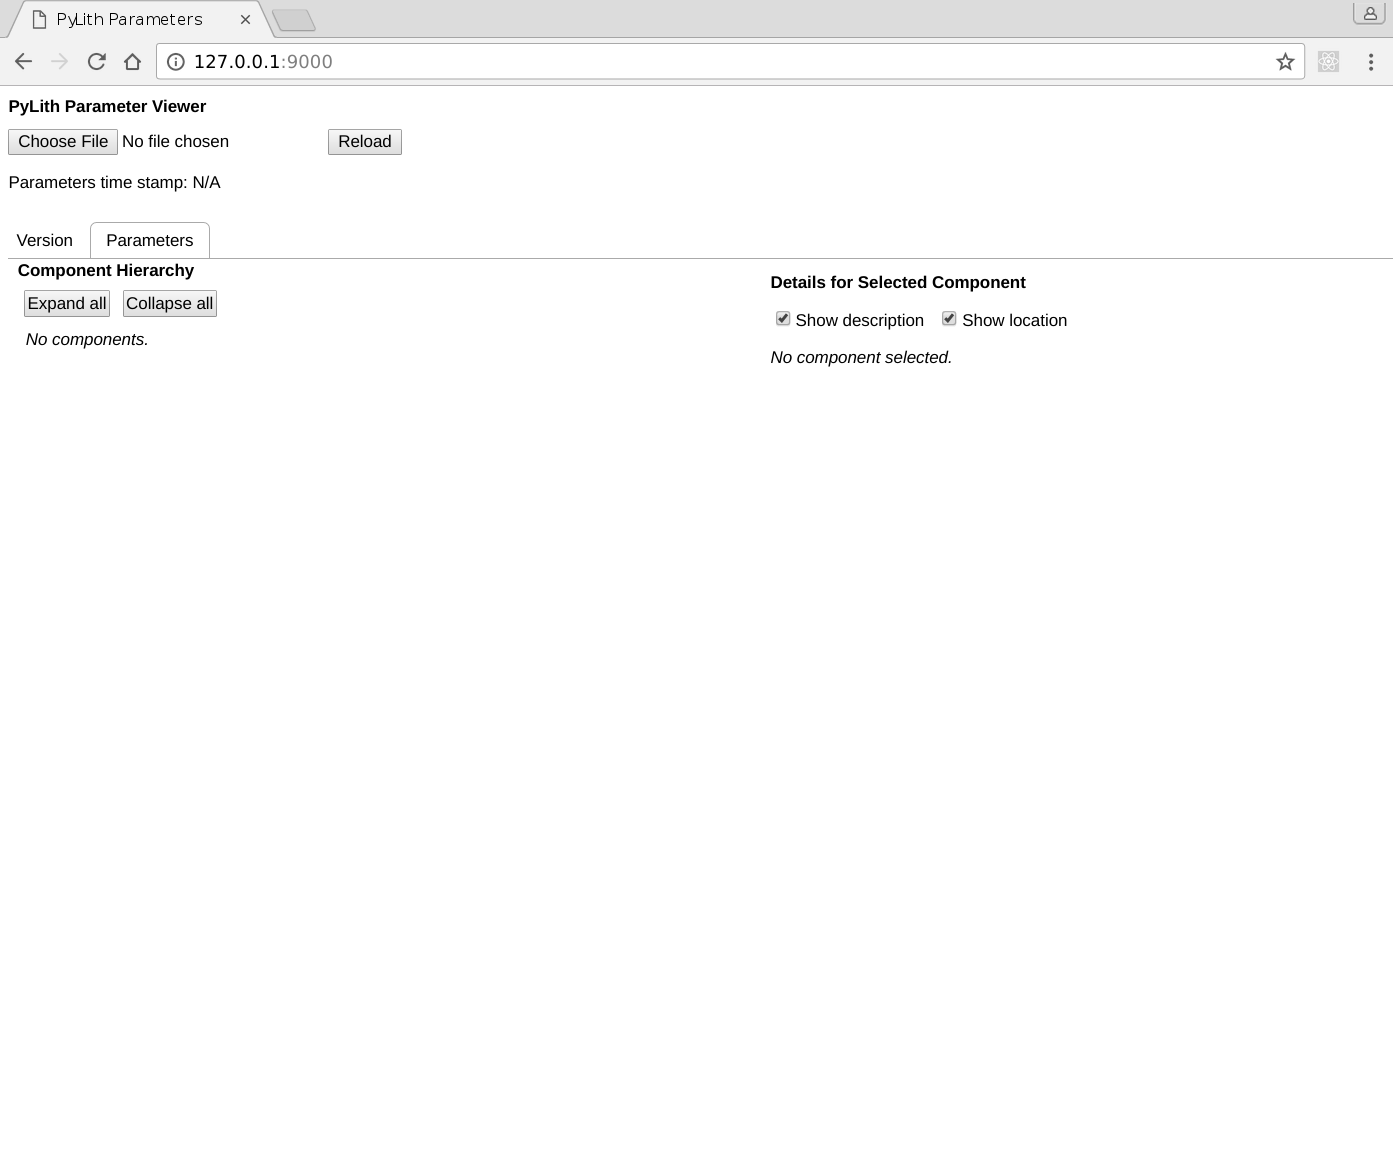
\includegraphics[width=5in]{runpylith/figs/paramgui_startup}}
  \caption{Screenshot of PyLith Parameter Viewer in web browser upon startup.}
  \label{fig:parameters:gui:startup} 
\end{figure}


\subsubsection{Version Information}

Click on the \textsf{Version} tab to examine the version information.
This tab displays the same version information shown with the
\filename{-{}-version} command line argument to \filename{pylith} in
an easy to read layout.  This includes information about the platform
on which \filename{pylith} or \filename{pylith\_info} was run, the
PyLith version, and versions of the dependencies, as shown in Figure
\ref{fig:parameters:gui:version}.

\begin{figure}[htbp]
  \fbox{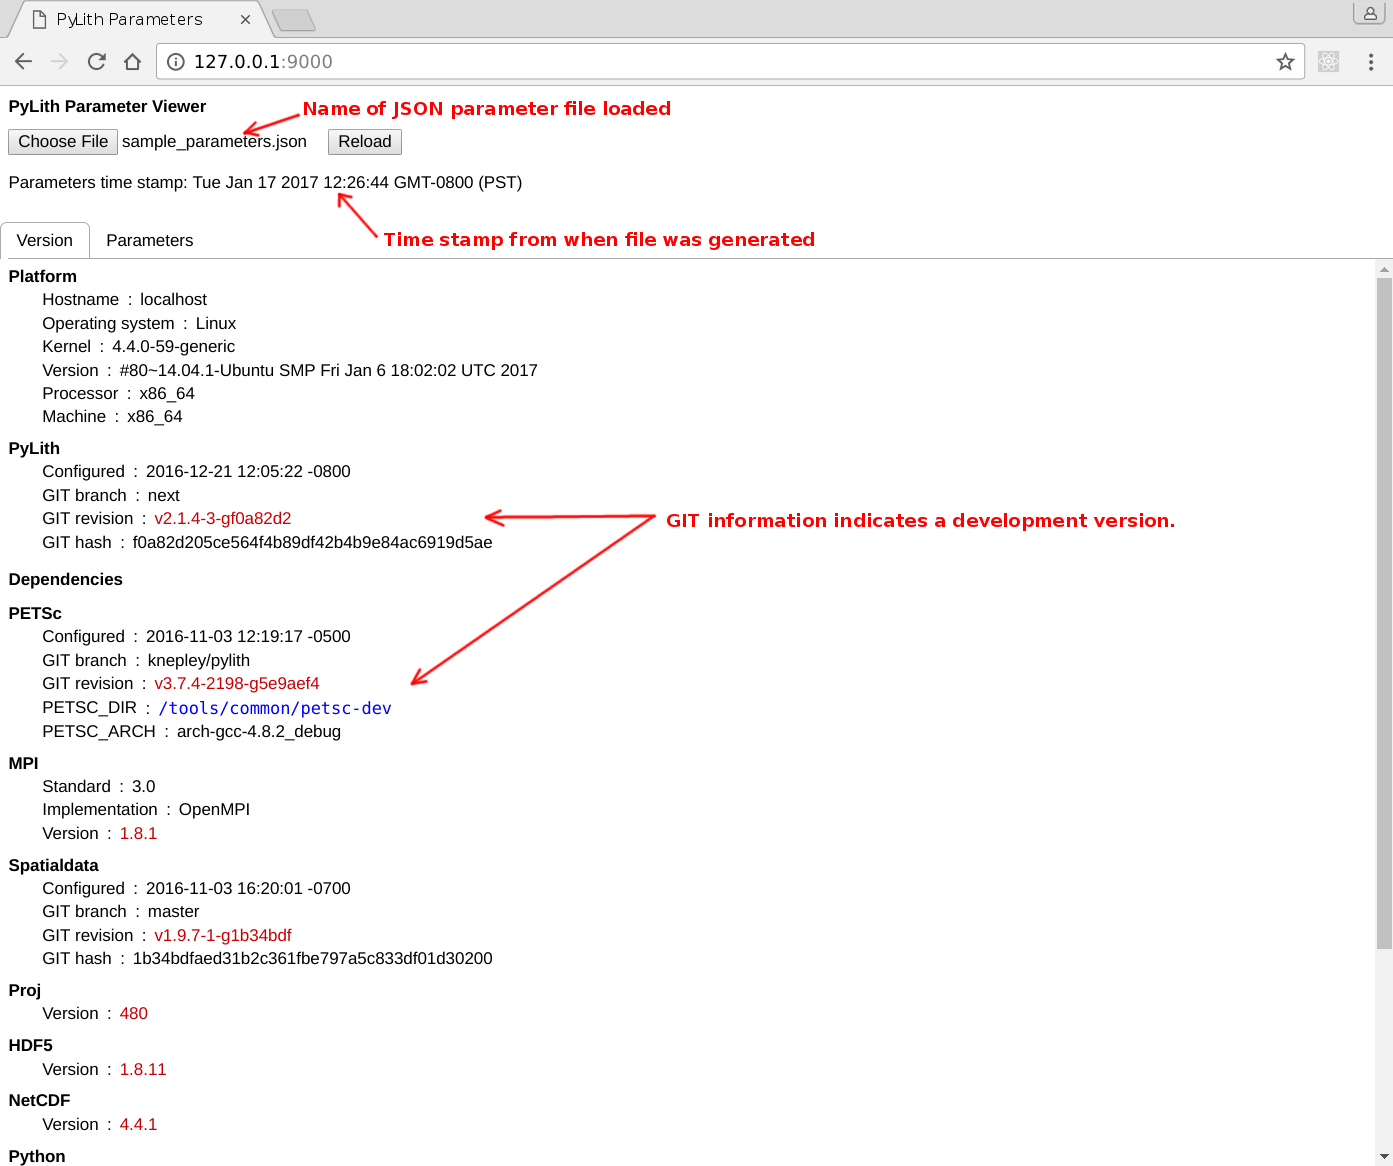
\includegraphics[width=5in]{runpylith/figs/paramgui_version}}
  \caption{Screenshot of \textsf{Version} tab of the PyLith Parameter Viewer
    with sample JSON parameter file.}
  \label{fig:parameters:gui:version} 
\end{figure}


\subsubsection{Parameter Information}

Click on the \textsf{Parameters} tab to examine the hiearchy of
components and the parameters for each. You can expand/collapse the
Component Hierarchy tree in the left panel by clicking on the
triangles or facility name in blue to the left of the equals sign
(Figure \ref{fig:parameters:gui:parameters:empty}).  Clicking on the
component in red to the right of the equals sign will show its
parameters in the right panel (Figure
\ref{fig:parameters:gui:parameters:empty}).  The selected facility in
the left panel whose parameters are shown in the right panel will be
highlighted via a gray background (Figure
\ref{fig:parameters:gui:parameters:selected}).

\begin{figure}[htbp]
  \fbox{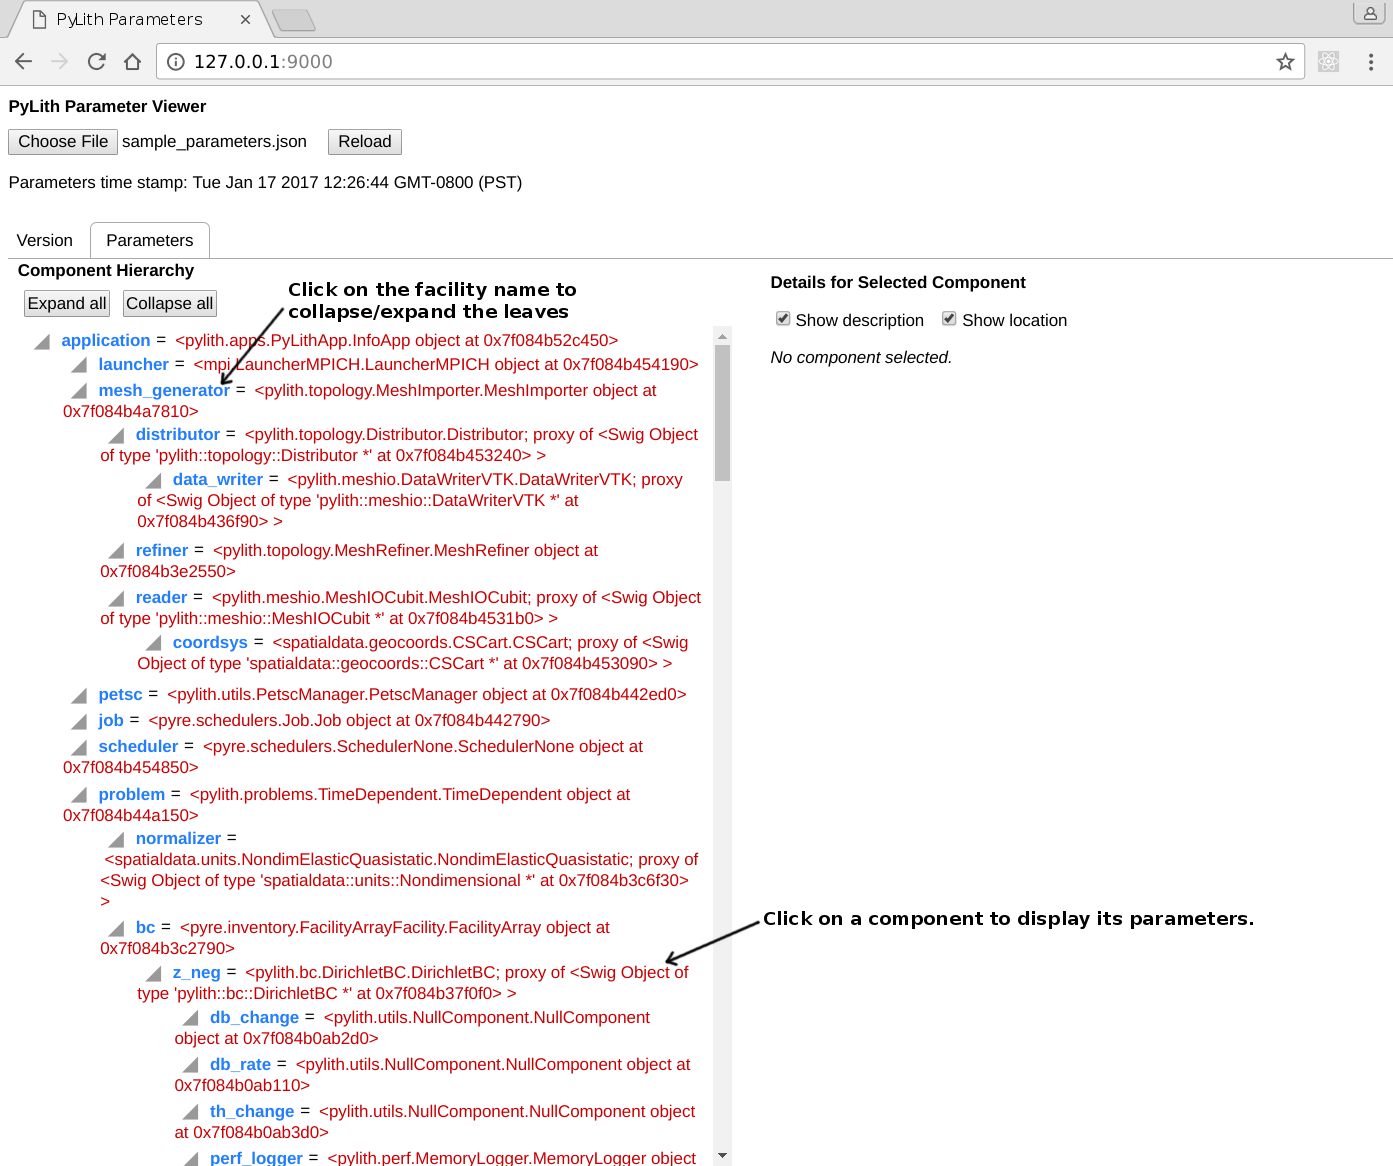
\includegraphics[width=5in]{runpylith/figs/paramgui_parameters}}
  \caption{Screenshot of \textsf{Parameters} tab of the PyLith Parameter Viewer
    with sample JSON parameter file before selecting a component in the
    left panel.}
  \label{fig:parameters:gui:parameters:empty}
\end{figure}


\begin{figure}[htbp]
  \fbox{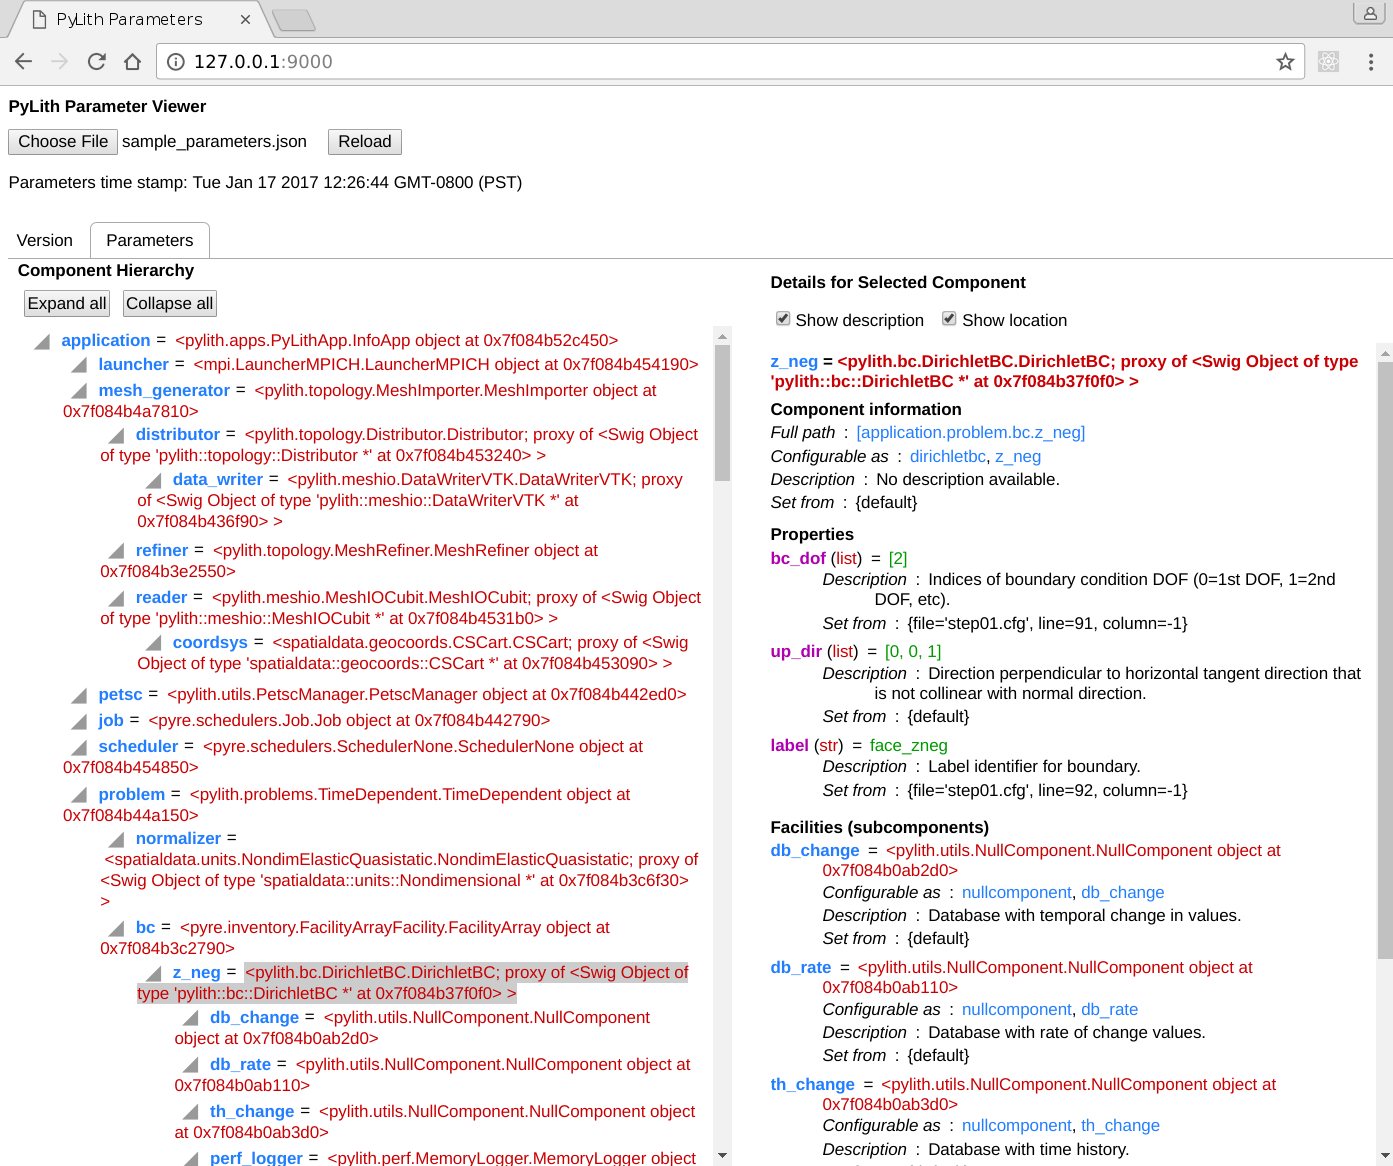
\includegraphics[width=5in]{runpylith/figs/paramgui_detail}}
  \caption{Screenshot of \textsf{Parameters} tab of the PyLith Parameter Viewer
    with sample JSON parameter file with the \facility{z\_neg} facility
    selected.}
  \label{fig:parameters:gui:parameters:selected} 
\end{figure}


% End of file

\input{./runpylith/troubleshooting.tex}

% End of file

